% !TeX spellcheck = en_GB
\section{Evaluation}
\subsection{Calibration}

\begin{figure}
	\centering
	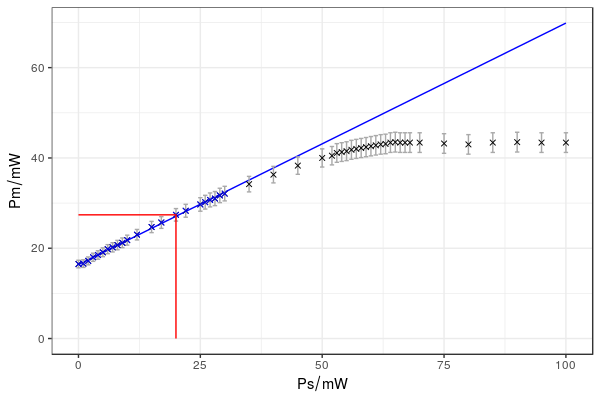
\includegraphics[width=\textwidth]{../figures/powercal.png}
	\caption{Measurement of the laser power}
	\label{fig:power}
\end{figure}

\begin{figure}
	\centering
	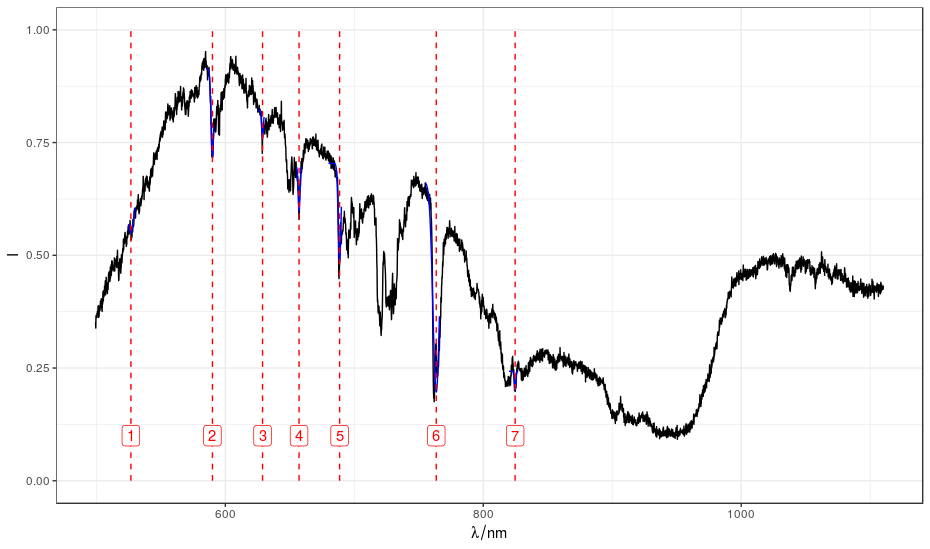
\includegraphics[width=\textwidth]{../figures/sunspectrum.png}
	\caption{Spectrum of the sun with identified Fraunhofer lines for calibration of the optical spectrometer}
	\label{fig:sunspectrum}
\end{figure}

\begin{table}
	\centering
	\begin{tabular}{c|c|c|c|c}
		Peak&Position&Element&Position \cite{fraunhoferlines}&Difference\\
		1&$526.8\pm1.7$&Fe I&527.0&$-0.2$\\
		2&$590.0\pm0.5$&Na I&589.6&$+0.4$\\
		3&$628.9\pm0.3$&Fe I&630.3&$-1.4$\\
		4&$657.2\pm0.3$&H $\alpha$&656.3&$+0.9$\\
		5&$688.6\pm0.5$&&&\\
		6&$763.5\pm1.3$&&&\\
		7&$824.7\pm0.3$&&&\\
	\end{tabular}
	\caption{Positions of the Fraunhofer Lines compared to the literature values}
\end{table}

\begin{figure}
	\centering
	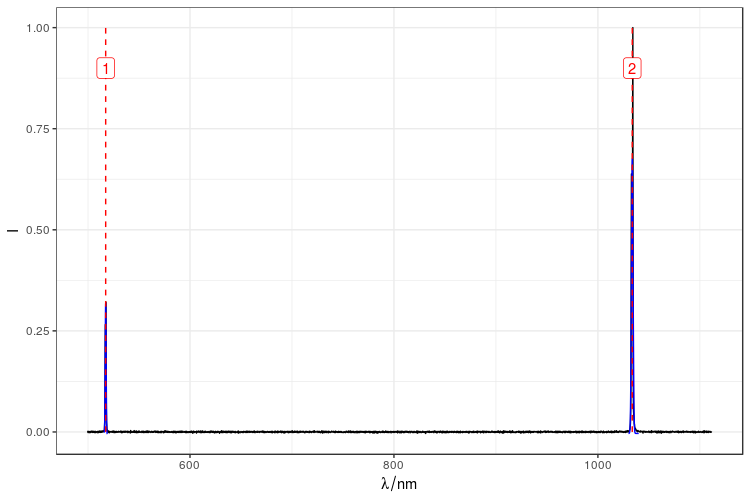
\includegraphics[width=\textwidth]{../figures/laserspectrum.png}
	\caption{Spectrum of the laser width identified peaks at the wavelengths $\lambda=(517.3\pm0.2)\,\mathrm{nm}$ and $\lambda=(1033.7\pm0.4)\,\mathrm{nm}$}
	\label{fig:laserspectrum}
\end{figure}

\subsection{Size of the Diamonds}

\subsection{Fluorescence Spectrum}

\subsection{ODMR Measurements}